\tikzstyle{line} = [draw, -latex']
\tikzstyle{vecArrowWhite} = [thick, decoration={markings,mark=at position
   1 with {\arrow[semithick]{open triangle 60}}},
   double distance=1.4pt, shorten >= 5.5pt,
   preaction = {decorate},
   postaction = {draw,line width=1.4pt, white, shorten >= 4.5pt}]
\tikzstyle{vecArrowGreen} = [thick, decoration={markings, mark=at position
   1 with {\arrow[semithick, fill=black]{triangle 60}}},
   postaction = {draw, line width=1.4pt, black, shorten >= 4.5pt}]
\tikzstyle{innerWhite} = [semithick, white,line width=1.4pt, shorten >= 4.5pt]
\tikzstyle{innerGreen} = [semithick, black, line width=1.4pt, shorten >= 4.5pt]


\newcolumntype{M}{>{\centering\arraybackslash}m{\dimexpr.35\linewidth-2\tabcolsep}}
\newtheorem{example}{Example}
\newtheorem{theorem}{Theorem}[section]
\newtheorem{lemma}{Lemma}[section]
\newtheorem{axiom}{Axiom}%[section]%[numberby]
\newcommand\tavan{\mathbin{\char`\^}}
%\newcommand{\tuple}[5]{$\langle$\textit{#1}, \textit{#2}, \textit{#3}, \textit{#4},
 %  \textit{#5} (explained in the latter)$\rangle$} \tuple{sourcelocation}{R/W}{tripcounter}{occurrence}{killed}
 \newcommand{\longtwopartdef}[4]
 {
 	\left\{
 		\begin{array}{ll}
 			\parbox{8cm}{$#1:$} &  #2 \\
 			\parbox{8cm}{$#3:$} &  #4
 		\end{array}
 	\right.
 }
\newcommand{\blankline}{\vspace{\baselineskip}}
\newcommand{\halflineup}{\vspace{-0.5\baselineskip}}
\newcommand{\qqquad}{\qquad\quad}
% general
\newcommand{\mesallossyfif}{\begin{tikzpicture}{every node}
 \node[point,label=left:$a$] (A) {};
           	   \node[point,right of=A,label=below:$b_1\ \ \ $, node distance=1cm] (B1) {};
           	   \node[point,right of=B1,label=below:$\ \ \ b_2$, node distance=0cm] (B2) {};
           	   \node[point,right of=B2,label=right:$c$, node distance=1.5cm] (C) {};
           	   \draw[lossysync] (A) to (B1);
           	   \draw[fifo] (B2) -- (C);
\end{tikzpicture}
}
\newcommand{\mesaldofilter}{\begin{tikzpicture}{every node}
 \node[point,label=left:$a$] (A) {};
  \node[right of=A, node distance=.85cm] (m1) {};
           	   \node[above of=m1,label=above:$p$, node distance=.1cm] (l1) {};
           	   \node[point,right of=A,label=below:$b_1\ \ \ $, node distance=1.5cm] (B1) {};
           	   \node[point,right of=B1,label=below:$\ \ \ b_2$, node distance=0cm] (B2) {};
           	   \node[point,right of=B2,label=right:$c$, node distance=1.5cm] (C) {};
           	     \node[right of=B1, node distance=.85cm] (m2) {};
           	   \node[above of=m2,label=above:$\neg p$, node distance=.1cm] (l2) {};
           	  % \draw[filter] (A) to (B1);
           	   %\draw[filter] (B2) to (C);
%  \filldraw [black] (0,0) circle (1pt) (1,0) circle (1pt);
       \draw [-, thick] (0,0) -- (0.5,0) -- (0.6, -0.1) -- (0.7, 0.1) -- (0.8, -0.1) -- (0.9, 0.1) --(0.95, 0);
       \draw [->, thick](0.95,0) -- (1.5,0);
% \filldraw [black] (1,0) circle (1pt) (1,0) circle (1pt);
       \draw [-, thick] (1.5,0) -- (2.05,0) -- (2.15, -0.1) -- (2.25, 0.1) -- (2.35, -0.1) -- (2.45, 0.1) --(2.55, 0);
       \draw [->, thick](2.55,0) -- (3,0);
\end{tikzpicture}
}
\newcommand{\reointerrupt}{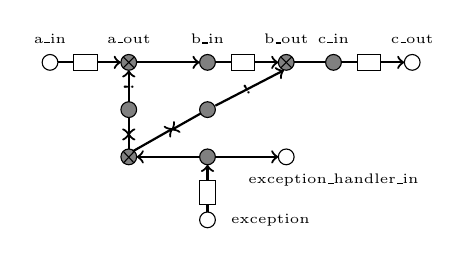
\begin{tikzpicture}{every node}=[font=\tiny]
\draw (0,0) ellipse (.1 and .1);
\node at (0,.3){a\_in};
\draw[fill=black!50] (1,0) ellipse (.1 and .1);
\node at (1,.3){a\_out};
\draw[->,thick](.1,0) -> (.9,0);
\draw[->,thick](1.1,0) -> (1.9,0);
\draw[fill=white] (.3,-.1) rectangle (.6,.1);
\draw[-](1.07,0.07) -- (.93,-0.07);
\draw[-](.93,0.07) -- (1.07,-0.07);
\begin{scope}[shift={(0,-.8)}]
%zire aout 
\draw[fill=black!50] (1,-0.4) ellipse (.1 and .1);
\node at (1,.3){};
\draw[-](1.07,-0.48) -- (.93,-0.33);
\draw[-](.93,-0.48) -- (1.07,-0.33);
\end{scope}
%syncdrain 1
\draw[->,thick](1,-1.1) -> (1,-.9);
\draw[->,thick](1,-.4) -> (1,-.93);
\draw[->,thick](1,-.7) -> (1,-.1);
\draw[fill=black!50] (1,-.6) ellipse (.1 and .1);
\node[rotate=90] at (1,-.32){\textbf{!}};
\begin{scope}[shift={(0,-3)}]
%exception
\draw (2,1) ellipse (.1 and .1);
\node at (2.8,1){exception};
\end{scope}
\begin{scope}[shift={(1,0)}]
\draw[->,thick](.9,-1.2) -> (.1,-1.2);
%balaye exception
\draw [fill=black!50](1,-1.2) ellipse (.1 and .1);
%exception
\draw(2,-1.2) ellipse (.1 and .1);
\draw[->,thick](1.1,-1.2) -> (1.9,-1.2);
\node at (2.6,-1.5){exception\_handler\_in};
\draw[->,thick](1,-1.9) -> (1,-1.3);
\draw[fill=white] (.9,-1.5) rectangle (1.1,-1.8);
\end{scope}
\begin{scope}[shift={(2,0)}]
%bin
\draw[fill=black!50]  (0,0) ellipse (.1 and .1);
\node at (0,.3){b\_in};
%bout
\draw[fill=black!50](1,0) ellipse (.1 and .1);
\node at (1,.3){b\_out};
\draw[->,thick](.1,0) -> (.9,0);
\draw[->,thick](1.1,0) -> (1.7,0);
\draw[fill=white] (.3,-.1) rectangle (.6,.1);
\draw[-](1.07,0.07) -- (.93,-0.07);
\draw[-](.93,0.07) -- (1.07,-0.07);
%syncdrain 2
\node[rotate=30] at (.5,-.35){\textbf{!}};
\draw[->,thick](-.95,-1.13) -> (-.44,-0.84);
\draw[->,thick](0,-0.6) -> (-.46,-0.86);
\draw[->,thick](.1,-.55)->(.97,-0.1);
\draw[fill=black!50](0,-0.6) ellipse (.1 and .1);
\end{scope}

\begin{scope}[shift={(3.6,0)}]
%cin
\draw[fill=black!50](0,0) ellipse (.1 and .1);
\node at (0,.3){c\_in};
%cout
\draw(1,0) ellipse (.1 and .1);
\node at (1,.3){c\_out};
\draw[->,thick](.1,0) -> (.9,0);
\draw[fill=white] (.3,-.1) rectangle (.6,.1);
\end{scope}
\end{tikzpicture}
}
\newcommand{\reointerruptbk}{ \begin{tikzpicture}[node distance = 2cm, auto,>=stealth]
               \node (writer) [abstract, rectangle split, rectangle split parts=2,text width=1.9cm, xshift=-2cm]
               {Writer
               \nodepart{second} \newline {requests=-1}\newline} ;
               \node[port, right of = writer, xshift = -9mm](M){};
               \node [draw,circle,minimum width=15pt, fill=black!50,xshift=26mm,left of=M](B){}; 
              \node[draw=none, right of = B,xshift=-7mm](C){};
           \draw[-, color=gray](M) -- (B);
            \draw[line](B) -> (C);
            
             \node [draw,circle,minimum width=15pt, fill=black!50,xshift=21mm,left of=C](B1){}; 
              \node[draw=none, right of = B1,xshift=-7mm](C1){};
           \node[right of=C1,xshift=-40.5mm](E){!};
            \node[right of=C1,xshift=-27mm](P){};
            \node[right of=C1,xshift=-26mm](Q){};
        %   \draw[line](B1) -> (Q);
           %\draw[line](C1) -> (P);    

%       \filldraw [black] (0,0) circle (1pt) (1,0) circle (1pt);
       \draw [->,thick] (1.35,-0.8) -- (1.8,-.8);
       \draw [->,thick] (2.4,-.8) -- (1.8,-.8);
      
         
         \node [draw,circle,minimum width=15pt, fill=black!50,xshift=-6mm,right of=B1](B2){}; 
           \node[right of=B2, xshift=-17.8mm,yshift=3.5mm](B3){};
	   \node[right of=B2, xshift=-22mm,yshift=3.5mm](B4){};
	    \node[right of=B2, xshift=-22mm,yshift=-3.5mm](B5){};
	   \node[right of=B2, xshift=-17.8mm,yshift=-3.5mm](B6){};
	  
	   \draw [-,thick] (2.34,-.99) -- (2.66,-.63);
       \draw [-,thick] (2.66,-0.99) -- (2.34,-.63);
	  % \draw[-,thick](B3) -- (B5);            
	  % \draw[-,thick](B4) -- (B6);            
	%\draw[line](B2) -> (C1); 
         \node [draw,circle,minimum width=15pt, fill=black!50,yshift=-5mm,above of=B2](B7){}; 
         \node [draw,circle,minimum width=15pt, fill=black!50,yshift=5mm,below of=B2](B8){}; 
      \draw[line](B7) -> (B2); 
      \draw[line](B2) -> (B8);    
      
\node[right of=B3, xshift=-19.5mm,yshift=5mm](B9){};
	   \node[right of=B3, xshift=-25mm,yshift=5mm](BA){};
	    \node[right of=B3, xshift=-19.5mm,yshift=1.1mm](BB){};
	   \node[right of=B3, xshift=-25mm,yshift=1.1mm](BC){};
	%   \draw[-,thick](BB) -- (BC) -- (BA) -- (B9)--(BB);
           \node[rectangle,fill=white, minimum width=1mm, draw=black,minimum height=6mm,xshift=25mm,yshift=.5mm](F){};
            \end{tikzpicture}}

% UMLAD
\newcommand{\realactivity}{ 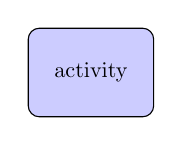
\begin{tikzpicture}[node distance = 0cm, auto, scale=.8, transform shape]
	                    % Place nodes
	                    \node [rectangle, draw, fill=blue!20, 
	                    text width=5em, text centered, rounded corners, minimum height=4em] (A) {};
	                    \node [left of=A,draw=none] (left) {};
	                    \node [draw=none, right of=A] (right) {};
	                    \node [left of=A,draw=none,xshift=0mm,yshift=0mm] (txt) {activity};
	                \end{tikzpicture}}
\newcommand{\umlactivity}{
	     \begin{tikzpicture}[node distance = 1cm, auto]
	                    % Place nodes
	                    \node [rectangle, draw, fill=blue!20, 
	                    text width=2.5em, text centered, rounded corners, minimum height=2em] (A) {};
	                    \node [left of=A,draw=none] (left) {};
	                    \node [draw=none, right of=A] (right) {};
	                    \node [left of=A,draw=none,xshift=10mm] (txt) {action};
	                    % Draw edges
	                    \path [line] (left) -- (A);
	                    \path [line] (A) -- (right);
	                \end{tikzpicture}}
	    
\newcommand{\umlactivitymore}{  \begin{tikzpicture}[scale=0.5,node distance = 1cm, auto]
	                           % Place nodes
	                           \node [rectangle, draw, fill=blue!20, 
	                           text width=3em, text centered, rounded corners, minimum height=2em] (init) {};
	                             \node [draw=none, right of=init] (system) {};
	                             \node [draw=none, below of=init,yshift=11mm,xshift=-4mm] (a) {};
	                              \node [draw=none, below of=init,yshift=10mm,xshift=-4mm] (b) {};
	                              \node [draw=none, below of=init,yshift=11mm,xshift=4mm] (c) {};
	                              \node [draw=none, below of=init,yshift=10mm,xshift=4mm] (d) {};
	                           \node [draw=none, above of=system,node distance=.5cm,yshift=-2mm] (upsystem) {};
	                            \node [draw=none, below of=system,node distance=.5cm,yshift=2mm] (downsystem) {};
	                          \node [draw=none, left of=init] (left) {};
	                           \node [draw=none, above of=left,node distance=.5cm,yshift=-2mm] (upleft) {};
	                            \node [draw=none, below of=left,node distance=.5cm,yshift=2mm] (downleft) {};                       
	                        % Draw edges
	                       %    \path [line] (left) -- (init);
	                               \path [line] (upleft) -- (a);
	                                   \path [line] (downleft) -- (b);
	                     %      \path [line] (init) -- (system);
	                           \path [line] (c) -- (upsystem);
	                           \path [line] (d) -- (downsystem);
	                            \node [draw=none, left of=init,xshift=1cm] (txt) {activity};
	      \end{tikzpicture}}
\newcommand{\umldatachanta}{\begin{tikzpicture}[scale=0.5,node distance = 2cm, auto]
	                           % Place nodes
	                           \node [rectangle, draw, fill=blue!20, 
	                           text width=5em, text centered,  minimum height=4em] (init) {};
	                             \node [draw=none, right of=init] (system) {};
	                             \node [draw=none, below of=init,yshift=21mm,xshift=-9mm] (a) {};
	                              \node [draw=none, below of=init,yshift=19mm,xshift=-9mm] (b) {};
	                              \node [draw=none, below of=init,yshift=21mm,xshift=9mm] (c) {};
	                              \node [draw=none, below of=init,yshift=19mm,xshift=9mm] (d) {};
	                           \node [draw=none, above of=system,node distance=1cm,yshift=-3mm] (upsystem) {};
	                            \node [draw=none, below of=system,node distance=1cm,yshift=3mm] (downsystem) {};
	                          \node [draw=none, left of=init] (left) {};
	                           \node [draw=none, above of=left,node distance=1cm,yshift=-3mm] (upleft) {};
	                            \node [draw=none, below of=left,node distance=1cm,yshift=3mm] (downleft) {};                       
	                        % Draw edges
	                       %    \path [line] (left) -- (init);
	                               \path [line] (upleft) -- (a);
	                                   \path [line] (downleft) -- (b);
	                     %      \path [line] (init) -- (system);
	                           \path [line] (c) -- (upsystem);
	                           \path [line] (d) -- (downsystem);
	      \end{tikzpicture}}
\newcommand{\umlinitalnode}{ \begin{tikzpicture}[scale=.5, transform shape, node distance = 2cm, auto]
       \draw [fill,black] (1.5,3) circle (.25cm);
        \draw[line](1.75,3)->(2.5,3);  
            \end{tikzpicture}}
\newcommand{\umlflow}{\begin{tikzpicture}
        \draw[line,thin](0,.5)->(.5,.5);    
         \end{tikzpicture}}
\newcommand{\umlacceptnode}{ \begin{tikzpicture}[node distance = 2cm, auto]
        \draw[line](.75,.25)->(1.2,.25);   
        \draw [line] (.15,.25) -- (0,.5) -- (.75,.5) -- (.75,0) -- (0,0) -- cycle;    
         \end{tikzpicture}}
\newcommand{\umlflowfinal}{     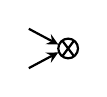
\begin{tikzpicture}[>=stealth, scale=.5, transform shape]
\draw[->, thick] (1.75,0.5) -- (2.5,0.1);
\draw[->, thick] (1.75,-0.5) -- (2.5,-0.1);
%\draw[->, thick] (1.5,0) -- (2.5,0);
\draw (2.75,0) ellipse (.25 and .25)[thick];
%\draw[->,thick](3,0) -- (3.75,0);
\draw[-,thick](2.6,0.2) -- (2.9,-0.2);
\draw[-,thick](2.6,-0.2) -- (2.9,0.2);
\end{tikzpicture}}
\newcommand{\umlmerge}{ \begin{tikzpicture}[node distance = 2cm, auto, scale=.5, transform shape]
             % Place nodes
            \node [decision] (decide) {};
             \node [draw=none, left of=decide,xshift=9mm] (left) {};
                 \node [draw=none, right of=decide,xshift=-10mm] (right) {};
                     \node [draw=none, above of=left,yshift=-15mm] (upright) {};
                         \node [draw=none, below of=left,yshift=15mm] (downright) {};
                        % \path [line] (left) -- (decide);
                                \path [line] (decide) -- (right);
                                      \path [line] (upright) -- (decide);
                                            \path [line] (downright) -- (decide);
         \end{tikzpicture} }
\newcommand{\umlfork}{\begin{tikzpicture}[node distance = 2cm, auto, scale=.5, transform shape]
             % Place nodes
            \node [fork] (decide) {};
             \node [draw=none, left of=decide,xshift=9mm] (left) {};
                 \node [draw=none, right of=decide,xshift=-9mm] (right) {};
                     \node [draw=none, above of=right,yshift=-10mm] (upright) {};
                         \node [draw=none, below of=right,yshift=10mm] (downright) {};
                         \path [line] (left) -- (decide);
                   %             \path [line] (decide) -- (right);
                                      \path [line] (decide) -- (upright);
                                            \path [line] (decide) -- (downright);
         \end{tikzpicture}}
\newcommand{\umldecision}{\begin{tikzpicture}[node distance = 2cm, auto, scale=.5, transform shape]
            % Place nodes
           \node [decision] (decide) {};
            \node [draw=none, left of=decide,xshift=1cm] (left) {};
                \node [draw=none, right of=decide,xshift=-5mm] (right) {};
                    \node [draw=none, above of=right,xshift=-3mm,yshift=-15mm] (upright) {};
                        \node [draw=none, below of=right,xshift=-3mm,yshift=15mm] (downright) {};
                        \path [line] (left) -- (decide);
			%			 \path [line] (decide) -- (right) node [near start,sloped,above] {\ \ \ \ cond2}(downright);
                         \path [line] (decide) -- (upright) node [near start,sloped,above] {\ \ \ \ cond1}(downright);
                         \path [line] (decide) -- (downright) node [near start,sloped, below] {\ \ \ \ cond2}(right);
        \end{tikzpicture}}
\newcommand{\umljoin}{\begin{tikzpicture}[node distance = 2cm, auto,scale=.5, transform shape]
              % Place nodes
             \node [fork] (decide) {};
              \node [draw=none, left of=decide,xshift=9mm] (left) {};
                  \node [draw=none, right of=decide,xshift=-9mm] (right) {};
                      \node [draw=none, above of=left,yshift=-9mm] (upright) {};
                          \node [draw=none, below of=left,yshift=9mm] (downright) {};
                        %  \path [line] (left) -- (decide);
                                 \path [line] (decide) -- (right);
                                       \path [line] (upright) -- (decide);
                                             \path [line] (downright) -- (decide);
          \end{tikzpicture}}
\newcommand{\umldatastore}{    \begin{tikzpicture}[node distance = .8cm, auto]
   \node [rectangle, draw, fill=blue!20, 
          text width=1em, text centered, minimum height=1.5em] (init) {};
          \node [left of=init,draw=none] (expert) {};
          \node [draw=none, right of=init] (system) {};
                 \path [line] (expert) -- (init);
                 \path [line] (init) -- (system);
   \end{tikzpicture}}
\newcommand{\umldatacomponent}{ \begin{tikzpicture}[node distance = 2cm, auto,scale=.5, transform shape]
                                % Place nodes
                                \node [rectangle, draw, fill=blue!20, 
                                text width=5em, text centered, minimum height=4em] (init) {};
                                  \node [draw=none, right of=init] (system) {};
                                \node [draw=none, above of=system,node distance=1cm] (upsystem) {};
                                 \node [draw=none, below of=system,node distance=1cm] (downsystem) {};
                               \node [draw=none, left of=init] (left) {};
                                \node [draw=none, above of=left,node distance=1cm] (upleft) {};
                                 \node [draw=none, below of=left,node distance=1cm] (downleft) {};                       
                             % Draw edges
                                \path [line] (left) -- (init);
                                    \path [line] (upleft) -- (init);
                                        \path [line] (downleft) -- (init);
                                \path [line] (init) -- (system);
                                \path [line] (init) -- (upsystem);
                                \path [line] (init) -- (downsystem);
           \end{tikzpicture}}
          \newcommand{\exedge}{\begin{tikzpicture}
             \draw [line,thin] (.35,.4) -- (.48,.4) -- (.35, .27)->(.78,.32);          
                       \end{tikzpicture}} 
           \newcommand{\cleanumlex}{\begin{tikzpicture}[cross/.style={path picture={  
                      \draw[black](path picture bounding box.south east) -- (path picture bounding box.north west) (path picture bounding box.south west) -- (path picture bounding box.north east);}}] 
                           \draw [line,thin] (.35,.4) -- (.48,.4) -- (.35, .27)->(.78,.32);
                                \begin{scope}[dashed]
                          \draw (-.25,0) -- (.5,0)-- (.5,.5) -- (-.25,.5) --cycle;
                          \end{scope}
                                   \end{tikzpicture}}
\newcommand{\umlsquare}{\begin{tikzpicture}
     \draw (0,0) -- (.15,0)-- (.15,.15) -- (0,.15) --cycle;
\end{tikzpicture}}   
\newcommand{\inpin}{\begin{tikzpicture}
     \draw[line] (-.6,.075)--(0,.075);
     \draw (0,0) -- (.15,0)-- (.15,.15) -- (0,.15) --cycle;
\end{tikzpicture}}    
\newcommand{\outpin}{
\begin{tikzpicture}
     \draw[line] (.15,.075)--(.75,.075);
     \draw (0,0) -- (.15,0)-- (.15,.15) -- (0,.15) --cycle;
\end{tikzpicture}}    
\newcommand{\umlexceptionstructure}{\begin{tikzpicture}[cross/.style={path picture={   \draw[black](path picture bounding box.south east) -- (path picture bounding box.north west) (path picture bounding box.south west) -- (path picture bounding box.north east);}}] 
    \node [rectangle, draw, fill=blue!20, 
           text width=5em, text centered, rounded corners, minimum height=4em] at (2,1) (init) {};
           \node [left of=init,draw=none] (expert) {};
           \node [draw=none, right of=init] (system) {};
           \draw [->] (3,2.5) -- (4.5,2.5);
            \draw [line] (1,2.5) -- (.5,3) -- (3,3) -- (3,2) -- (.5,2) -- cycle;    
            \draw [line] (3.5,2.9) -- (3.8,2.9) -- (3.5, 2.7)->(3.8,2.7);
            \node [rectangle, draw, fill=blue!20, 
           text width=5em, text centered, rounded corners, minimum height=4em] at (5.5,2.4) (ex) {};
            \begin{scope}[thick,dashed]
    \draw (0,0) -- (4,0)-- (4,3.5) -- (0,3.5) --cycle;
    \end{scope}
             \end{tikzpicture}}
\newcommand{\umlactivityfinal}{
          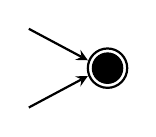
\begin{tikzpicture}[>=stealth]
\draw[->, thick] (1.75,0.5) -- (2.5,0.1);
\draw[->, thick] (1.75,-0.5) -- (2.5,-0.1);
%\draw[->, thick] (1.5,0) -- (2.5,0);
\draw (2.75,0) ellipse (.25 and .25)[thick];
 \node [draw,circle,xshift=-2.5mm,,minimum width=11pt,fill](M) at (3,0){};
        \end{tikzpicture}}
\newcommand{\umltimer}{\begin{tikzpicture}[node distance = 1cm, auto]    
\draw [line] node [left, node distance=1cm] {$t \ \ $}(0,0) -- (-.25,.25) -- (.25,.25) -- cycle;
\draw [line] (0,0) -- (-.25,-.25) -- (.25,-.25) -- cycle;
\draw[line](0,0)->(.5,0);
\end{tikzpicture}}
%uml2Reo
\newcommand{\reodatayek}{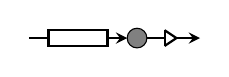
\begin{tikzpicture}[>=stealth, scale=.5, transform shape]
\draw[-, thick] (0,0) -- (.5,0);
\draw [thick](.5,.2) rectangle (2,-.2);
\draw[->, thick] (2,0) -- (2.5,0);
\draw (2.75,0) ellipse (.25 and .25)[fill=gray];
\draw[-,thick](3,0) -- (3.45,0);
\draw[-,thick](3.45,-.2) -- (3.45,.2);
\draw[-,thick](3.45,-.2) -- (3.75,0);
\draw[-,thick](3.45,.2) -- (3.75,0);
\draw[->,thick](3.75,0) -> (4.35,0);
\end{tikzpicture}}
\newcommand{\reotimer}{ 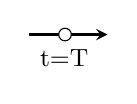
\begin{tikzpicture}[>=stealth]
       \def\rectanglepath{-- ++(0.5cm,0cm) -- ++(0cm,0.2cm) -- ++(-0.5cm,0cm) -- cycle}
  		\draw [->, thick] (0,0) -- (1,0);
        \draw (.46,0) ellipse (.08 and .08)[fill=white];
		\node[font=\small] at (.45,-0.3) {t=T};
    \end{tikzpicture}}
\newcommand{\reotimerbk}{       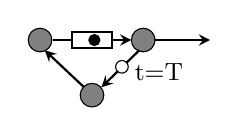
\begin{tikzpicture}[>=stealth]
       \filldraw [black] (0.53,0) circle (2pt) (1,0);
       \def\rectanglepath{-- ++(0.5cm,0cm) -- ++(0cm,0.2cm) -- ++(-0.5cm,0cm) -- cycle}
       \draw [thick] (0.25,-0.1) \rectanglepath;
       \draw [-, thick] (0,0) -- (0.25,0);
       \draw [->, thick](0.75,0) -- (1,0);
       \draw (-0.16,0) ellipse (.15 and .15)[fill=gray];
		\draw (1.15,0) ellipse (.15 and .15)[fill=gray];
	    \draw (.5,-0.7) ellipse (.15 and .15)[fill=gray];
		\draw [->, thick] (1.1,-0.13) -- (0.62,-.6);
        \draw [->, thick](0.4,-.6) -- (-.1,-0.13);
        \draw (.88,-0.34) ellipse (.08 and .08)[fill=white];
		\draw [->, thick](1.3,0) -- (2,0);
		\node[font=\small] at (1.35,-0.4) {t=T};
    \end{tikzpicture}}
    \newcommand{\reocondition}{
    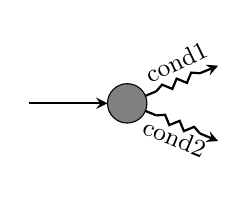
\begin{tikzpicture}[>=stealth]
        \draw[->, thick] (1.5,0) -- (2.5,0);
        \draw (2.75,0) ellipse (.25 and .25)[fill=gray];
        %
       % \node[font=\small] at (3.5,0.15) {cond2};
       % \draw[-,thick](3,0) -- (3.15,0);
        %\draw[->,thick](3.75,0) -- (4,0);
        %\draw[-,thick] (3.15,0) -- (3.25,0.05) -- (3.35,-0.05) -- (3.45,0.05)--(3.55,-0.05)--(3.65,0.05)--(3.75,0);        
        %
        \node[font=\small,rotate around={-22.5:(2,0)}] at (3.2,-1.2) {cond2};
        \draw[-,thick,rotate around={22.5:(2.75,0)}](3,0) -- (3.15,0);
        \draw[->,thick,rotate around={22.5:(2.75,0)}](3.75,0) -- (4,0);
        \draw[-,thick,rotate around={22.5:(2.75,0)}] (3.15,0) -- (3.25,0.05) -- (3.35,-0.05) -- (3.45,0.05)--(3.55,-0.05)--(3.65,0.05)--(3.75,0);
        %
        \node[font=\small,rotate around={25.5:(.75,0)}] at (3.3,0.85) {cond1};
        \draw[-,thick,rotate around={-22.5:(2.75,0)}](3,0) -- (3.15,0);
        \draw[-,thick,rotate around={-22.5:(2.75,0)}] (3.15,0) -- (3.25,0.05) -- (3.35,-0.05) -- (3.45,0.05)--(3.55,-0.05)--(3.65,0.05)--(3.75,0);
        \draw[->,thick,rotate around={-22.5:(2.75,0)}](3.75,0) -- (4,0);
        \end{tikzpicture}
    }
% REO
\newcommand{\componentdo}{ \begin{tikzpicture}[scale=.55, transform shape]
                  \node (writer) [abstract, rectangle split, rectangle split parts=2]
                  {component
                  \nodepart{second} \newline\newline\newline} ;
                     \node[port, left of = writer,xshift=1mm,yshift=0mm](M){};
             \node [draw,circle, fill=black!50, left of = M,xshift=.5cm](B){}; 
                     \node[draw=none, left of = B](C){};
              \draw[-, color=gray](M) -- (B);
               \draw[line,thick](C) -> (B);
                 %1
                  \node[port, below of = M,yshift=5mm](M1){};
             \node [draw,circle, fill=black!50, left of = M1,xshift=.5cm](B1){}; 
                    \node[draw=none, left of = B1](C1){};
              \draw[-, color=gray](M1) -- (B1);
               \draw[line,thick](C1) -> (B1);
               %right hand side
                 \node[port, right of = M,xshift=8mm](MM){};
             \node [draw,circle, fill=black!50, right of = MM,xshift=-5mm](BB){}; 
                     \node[draw=none, right of = BB](CC){};
              \draw[-, color=gray](MM) -- (BB);
               \draw[line,thick](BB) -> (CC);
                 %1
              \node[port, right of = M1,xshift=8mm](MM1){};
             \node [draw,circle, fill=black!50, right of = B1,xshift=18mm](BB1){}; 
              \node[draw=none, right of = BB1](CC1){};
              \draw[-, color=gray](MM1) -- (BB1);
               \draw[line,thick](BB1) -> (CC1);
            \end{tikzpicture}}
\newcommand{\component}{ \begin{tikzpicture}
                  \node (writer) [abstract, rectangle split, rectangle split parts=2]
                  {component
                  \nodepart{second} \newline\newline\newline} ;
                     \node[port, left of = writer,xshift=1mm,yshift=-2mm](M){};
             \node [draw,circle, fill=black!50, left of = M,xshift=.5cm](B){}; 
                     \node[draw=none, left of = B](C){};
              \draw[-, color=gray](M) -- (B);
               \draw[line,thick](C) -> (B);
                 %1
                  \node[port, below of = M,yshift=5mm](M1){};
             \node [draw,circle, fill=black!50, left of = M1,xshift=.5cm](B1){}; 
                    \node[draw=none, left of = B1](C1){};
              \draw[-, color=gray](M1) -- (B1);
               \draw[line,thick](C1) -> (B1);
           %2
              \node[port, above of = M,yshift=-5mm](M2){};
             \node [draw,circle, fill=black!50, left of = M2,xshift=.5cm](B2){}; 
                    \node[draw=none, left of = B2](C2){};
              \draw[-, color=gray](M2) -- (B2);
               \draw[line,thick](C2) -> (B2);
               %right hand side
                 \node[port, right of = M,xshift=8mm](MM){};
             \node [draw,circle, fill=black!50, right of = MM,xshift=-5mm](BB){}; 
                     \node[draw=none, right of = BB](CC){};
              \draw[-, color=gray](MM) -- (BB);
               \draw[line,thick](BB) -> (CC);
                 %1
              \node[port, right of = M1,xshift=8mm](MM1){};
             \node [draw,circle, fill=black!50, right of = B1,xshift=18mm](BB1){}; 
              \node[draw=none, right of = BB1](CC1){};
              \draw[-, color=gray](MM1) -- (BB1);
               \draw[line,thick](BB1) -> (CC1);
           %2
              \node[port, right of = M2,xshift=8mm](MM2){};
             \node [draw,circle, fill=black!50, right of =B2,xshift=18mm](BB2){}; 
                    \node[draw=none, right of = BB2](CC2){};
             \draw[-, color=gray](MM2) -- (BB2);
              \draw[line,thick](BB2) -> (CC2);
            \end{tikzpicture}}
\newcommand{\writer}{
              \begin{tikzpicture}[,scale=.5 ,transform shape, node distance = 2cm, auto]
               \node (writer) [abstract, rectangle split, rectangle split parts=2,text width=1.9cm, xshift=-2cm]
               {Writer
               \nodepart{second} \newline {requests=-1}\newline} ;
               \node[port, right of = writer, xshift = -9mm](M){};
               \node [draw,circle,minimum width=15pt, fill=black!50,xshift=26mm,left of=M](B){}; 
              \node[draw=none, right of = B,xshift=-7mm](C){};
           \draw[-, color=gray](M) -- (B);
            \draw[line](B) -> (C);
              \end{tikzpicture}
        }
      \newcommand{\reader}{   \begin{tikzpicture}[node distance = 2cm, auto, scale=.5, transform shape]
                  \node (writer) [abstract, rectangle split, rectangle split parts=2,text width=19mm]
                   {Reader
                   \nodepart{second} \newline {requests=-1}\newline} ;
                   \node[port, left of = writer, xshift = 9mm,yshift=2mm](M){};
                      \node [draw,circle,minimum width=15pt, fill=black!50,left of=M,xshift=13mm](B){}; 
                  \node[draw=none, left of = B,xshift=7mm](C){};
               \draw[-, color=gray](M) -- (B);
                \draw[line](C) -> (B);
                  \end{tikzpicture}
      }
\newcommand{\mergerNodeNamed}[3]{\tikz{
	    \node[inner sep=0,label=right:$#3$] (D1) {};
	    \node[point,left of=D1,node distance=4mm] (C1) {};
	    \node[inner sep=0,label=left:$#1$,above left of=C1,node
            distance=4mm] (B1) {};
	    \node[inner sep=0,label=left:$#2$,below left of=C1,node
            distance=4mm] (A1) {};
	    \draw[sync] (C1) to (D1);
	    \draw[channel] (A1) to (C1);
	    \draw[channel] (B1) to (C1); }}
\newcommand{\mergerNodeNamedabc}{\tikz[baseline={([yshift={-\ht\strutbox}]current bounding box.north)},outer sep=0pt,inner sep=0pt]{
	    \node[inner sep=0] (C1) {};
	    \node[inner sep=0, right of=C1, node distance=1.5mm] (CC1) {};
	    \node[inner sep=0,right of=C1,node distance=6mm,label=right:$c$] (D1) {};	    
        \node[inner sep=0,right of=C1,node distance=.8mm] (D2) {};
	    \node[inner sep=0,above left of=D2,node distance=0.8mm] (C2) {};
	    \node[inner sep=0,below left of=D2,node distance=0.8mm] (C3) {};
	    \node[inner sep=0,label=left:$a$,above left of=C2,node distance=4mm] (A1) {};
	    \node[inner sep=0,label=left:$b$,below left of=C3,node distance=4mm] (B1) {};
	    \draw[sync] (CC1) to (D1);
	    \draw[channel] (A1) to (C2);
	    \draw[channel] (B1) to (C3);
        \draw [-, thick] (0.08, 0) circle (3pt);
              \draw [-, thick](.083, -0.1) -- (.083,0.1);
        \draw [-, thick](0.009, 0) -- (0.55, 0);
      
       }}
\newcommand{\replicatorNodeNamedabc}{\tikz{
	    \node[inner sep=0,label=left:$a$] (D1) {};
	    \node[point,right of=D1,node distance=4mm] (C1) {};
	    \node[inner sep=0,label=right:$b$,above right of=C1,node
          distance=4mm] (B1) {};
	    \node[inner sep=0,label=right:$c$,below right of=C1,node
          distance=4mm] (A1) {};
	    \draw[channel] (D1) to (C1);
	    \draw[sync] (C1) to (A1);
	    \draw[sync] (C1) to (B1); }}
\newcommand{\replicatorNodeNamed}{\tikz{
	    \node[inner sep=0,label=left:$A$] (D1) {};
	    \node[point,right of=D1,node distance=4mm] (C1) {};
	    \node[inner sep=0,label=right:$B$,above right of=C1,node
          distance=4mm] (B1) {};
	    \node[inner sep=0,label=right:$C$,below right of=C1,node
          distance=4mm] (A1) {};
	    \draw[channel] (D1) to (C1);
	    \draw[sync] (C1) to (A1);
	    \draw[sync] (C1) to (B1); }}
\newcommand{\routerNodeNamed}{\tikz{
	    \node[inner sep=0,label=left:$A$] (D1) {};
	    \node[inner sep=0,right of=D1,node distance=4mm] (C1) {};
        \node[inner sep=0,right of=C1,node distance=1mm] (D2) {};
	    \node[inner sep=0,above right of=D2,node distance=1mm] (C2) {};
	    \node[inner sep=0,below right of=D2,node distance=1mm] (C3) {};
	    \node[inner sep=0,label=right:$B$,above right of=C2,node
          distance=4mm] (A1) {};
	    \node[inner sep=0,label=right:$C$,below right of=C3,node
          distance=4mm] (B1) {};
	    \draw[channel] (D1) to (C1);
	    \draw[sync] (C2) to (A1);
	    \draw[sync] (C3) to (B1);
        \draw [-, thick] (0.5, 0) circle (3pt);
        \draw [-, thick](0.43, -0.07) -- (0.57,0.07);
        \draw [-, thick](0.43, 0.07) -- (0.57, -0.07);
       }}

\newcommand{\syncNamed}[2]{
    \begin{tikzpicture}[>=stealth]
       \filldraw [black] (0,0) circle (1pt) (1,0) circle (1pt);
       \node[] at (-0.2,.2) {#1};
       \node[] at (1.2,.2) {#2};
       \draw [->,thick] (0,0) -- (1,0);
    \end{tikzpicture}
}
\newcommand{\psync}{
    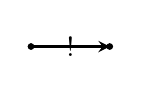
\begin{tikzpicture}[>=stealth]
       \filldraw [black] (0,0) circle (1pt) (1,0) circle (1pt);
       \draw [->,thick] (0,0) -- (1,0);
       \node[] at (0.5,0) {$!$};
    \end{tikzpicture}  
}

\newcommand{\bcsync}{
    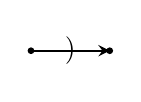
\begin{tikzpicture}[>=stealth]
       \filldraw [black] (0,0) circle (1pt) (1,0) circle (1pt);
       \draw [->,thick] (0,0) -- (1,0);
       \node[] at (0.5,0) {$)$};
    \end{tikzpicture}  
}


\newcommand{\bksync}{
    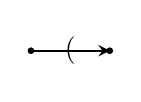
\begin{tikzpicture}[>=stealth]
       \filldraw [black] (0,0) circle (1pt) (1,0) circle (1pt);
       \draw [->,thick] (0,0) -- (1,0);
       \node[] at (0.5,0) {$($};
    \end{tikzpicture}  
}

\newcommand{\bsync}{
    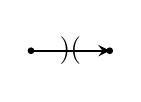
\begin{tikzpicture}[>=stealth]
       \filldraw [black] (0,0) circle (1pt) (1,0) circle (1pt);
       \draw [->,thick] (0,0) -- (1,0);
       \node[] at (0.5,0) {$)($};
    \end{tikzpicture}  
}
\newcommand{\syncdrain} {
    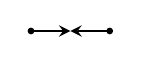
\begin{tikzpicture}[>=stealth]
       \filldraw [black] (0,0) circle (1pt) (1,0) circle (1pt);
       \draw [->,thick] (0,0) -- (0.5,0);
       \draw [->,thick] (1,0) -- (0.5,0);
    \end{tikzpicture}
}

\newcommand{\syncdrainab} {
    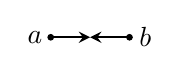
\begin{tikzpicture}[>=stealth]
       \filldraw [black] (0,0) circle (1pt) (1,0) circle (1pt);
       \draw [->,thick] (0,0) -- (0.5,0);
       \draw [->,thick] (1,0) -- (0.5,0);
                   \draw (-0.2,0) node [inner sep=0] {$a$};
        \draw (1.2,0) node [inner sep=0] {$b$};
    \end{tikzpicture}
}

\newcommand{\replicate}{
    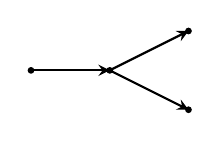
\begin{tikzpicture}[>=stealth]
       \filldraw [black] (0,0) circle (1pt) (1,0) circle (1pt) (2,0.5) circle (1pt) (2,-0.5) circle (1pt);
       \draw [->, thick] (0,0) -- (1,0);
       \draw [->, thick] (1,0) -- (2,0.5);
       \draw [->, thick] (1,0) -- (2,-0.5);
    \end{tikzpicture}
}

\newcommand{\mergeNode}{
    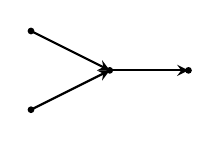
\begin{tikzpicture}[>=stealth]
       \filldraw [black] (0,0) circle (1pt) (1,0) circle (1pt) (-1,0.5) circle (1pt) (-1,-0.5) circle (1pt);
       \draw [->, thick] (-1, 0.5) -- (0,0);
       \draw [->, thick] (0,0) -- (1,0);
       \draw [->, thick] (-1,-0.5) -- (0,0);
    \end{tikzpicture}
}

\newcommand{\route}{
    \begin{tikzpicture}[>=stealth]
          \node[inner sep=0, label=left:$A$] at (0, 0)   (A)   {};
          \node[point]  at (0.5, 0)    (X1) {};
          \node[point]  at  (1.5,0.5)  (X2) {};
          \node[point]  at  (1.5,-0.5) (X3) {};
          \node[point]  at  (1.5,0)    (X4) {};
          \node[inner sep=0, label=right:$B$] at (2,0.5) (B) {};
          \node[inner sep=0, label=right:$C$] at (2,-0.5)(C) {};
          \draw[sync] (A) to (X1);
          \draw[lossysync] (X1) to (X2);
          \draw[lossysync] (X1) to (X3);
          \draw[syncdrain] (X1) to (X4);
          \draw[sync] (X2) to (X4);
     	  \draw[sync] (X3) to (X4);
          \draw[sync] (X2) to (B);
     	  \draw[sync] (X3) to (C);
    \end{tikzpicture}
}

\newcommand{\decomposedRoute}{
\small{
    \begin{tikzpicture}[>=stealth]
          \node[inner sep=0, label=left:$A$] at (0, 0) (A)   {};
          \node[point]  at (0.2, 0) (X1) {};

          \node[inner sep=0, label=above right:$D_1$] at  (0.4,0.2)  (D1) {};
          \node[inner sep=0, label=below right:$F_1$] at  (0.4,-0.2) (F1) {};
          \node[inner sep=0, label=right:$H_1$] at  (0.4,0)    (H1) {};

          \node[inner sep=0, label=left:$D_2$]  at  (1.5, 0.5)  (D2) {};
          \node[inner sep=0, label=left:$F_2$]  at  (1.5, -0.5) (F2) {};
          \node[inner sep=0, label=left:$H_2$]  at  (1.5, 0)   (H2) {};

          \node[inner sep=0, label=right:$E_2$]  at  (2.5,1)  (E2) {};
          \node[inner sep=0, label=right:$G_2$]  at  (2.5,-1) (G2) {};
          \node[inner sep=0, label=right:$K_2$]  at  (2.5,0)  (K2) {};

          \node[inner sep=0, label=left:$E_1$]  at  (3.6,1.3)  (E1) {};
          \node[inner sep=0, label=left:$G_1$]  at  (3.6,-1.3) (G1) {};
          \node[inner sep=0, label=left:$K_1$]  at  (3.6,0)    (K1) {};

          \node[point]  at  (3.8,1.4)  (X2) {};
          \node[point]  at  (3.8,-1.4) (X3) {};
          \node[point]  at  (3.8,0)    (X4) {};

          \node[inner sep=0, label=right:$J_1$]  at  (3.8,1.2)    (J1) {};
          \node[inner sep=0, label=right:$L_1$]  at  (3.8,-1.2)   (L1) {};
          \node[inner sep=0, label=left:$J_2$]  at  (3.8,1)    (J2) {};
          \node[inner sep=0, label=left:$L_2$]  at  (3.8,-1)   (L2) {};
          \node[inner sep=0, label=right:$I_1$]  at  (3.8,0.2)  (I1) {};
          \node[inner sep=0, label=right:$M_1$]  at  (3.8,-0.2) (M1) {};
          \node[inner sep=0, label=left:$I_2$]  at  (3.8,0.4)  (I2) {};
          \node[inner sep=0, label=left:$M_2$]  at  (3.8,-0.4) (M2) {};

          \node[inner sep=0, label=right:$B$]  at  (4,1.4)  (B) {};
          \node[inner sep=0, label=right:$C$]  at  (4,-1.4) (C) {};

          \draw[channel] (A) to (X1);
          \draw[channel] (X1) to (D1);
          \draw[channel] (X1) to (F1);
          \draw[channel] (X1) to (H1);

          \draw[lossysync] (D2) to (E2);
          \draw[lossysync] (F2) to (G2);
          \draw[syncdrain] (H2) to (K2);

          \draw[channel] (E1) to (X2);
          \draw[channel] (G1) to (X3);
          \draw[channel] (K1) to (X4);

          \draw[channel] (X4) to (I1);
          \draw[channel] (X4) to (M1);

          \draw[channel] (X2) to (J1);
          \draw[channel] (X3) to (L1);
          \draw[channel] (X2) to (B);
     	  \draw[channel] (X3) to (C);

          \draw[sync] (J2) to (I2);
          \draw[sync] (L2) to (M2);

    \end{tikzpicture}
}
}

\newcommand{\routeNodeSimple}{
    
\begin{tikzpicture}[>=stealth]
       \draw [-, thick] (0,0) circle (3pt);
       \draw [-, thick](-0.07, -0.07) -- (0.07,0.07);
       \draw [-, thick](-0.07, 0.07) -- (0.07, -0.07);
    \end{tikzpicture}
}


\newcommand{\reomerger}{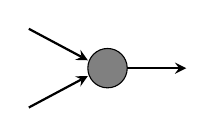
\begin{tikzpicture}[>=stealth]
\draw[->, thick] (1.75,0.5) -- (2.5,0.1);
\draw[->, thick] (1.75,-0.5) -- (2.5,-0.1);
%\draw[->, thick] (1.5,0) -- (2.5,0);
\draw (2.75,0) ellipse (.25 and .25)[fill=gray];
\draw[->,thick](3,0) -- (3.75,0);
\end{tikzpicture}}
\newcommand{\joinNodeWithdrieineenout}{
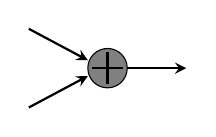
\begin{tikzpicture}[>=stealth]
\draw[->, thick] (1.75,0.5) -- (2.5,0.1);
\draw[->, thick] (1.75,-0.5) -- (2.5,-0.1);
%\draw[->, thick] (1.5,0) -- (2.5,0);
\draw (2.75,0) ellipse (.25 and .25)[fill=gray];
\draw[->,thick](3,0) -- (3.75,0);
\draw[-,thick](2.55,0) -- (2.95,0);
\draw[-,thick](2.75,.2) -- (2.75,-.2);
\end{tikzpicture}
}
\newcommand{\replicatorwithdireineenout}{
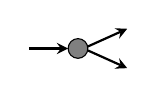
\begin{tikzpicture}[>=stealth,scale=.5, transform shape]
\draw[->, thick] (3,.05) -- (4,0.5);
\draw[->, thick] (3,-.05) -- (4,-0.5);
\draw[->, thick] (1.5,0) -- (2.5,0);
\draw (2.75,0) ellipse (.25 and .25)[fill=gray];
%\draw[->,thick](3,0) -- (4,0);
\end{tikzpicture}}
%Constraint Automata

\newcommand{\casync}{
    \begin{tikzpicture}[->,>=stealth',shorten >=1pt,auto,node distance=1.8cm,semithick]
      \tikzstyle{every state}=[draw=black,text=black,minimum size=10pt]
      \node[state] (s1) {};
      \path (s1) edge [loop right] node {$\{A,B\}$} (s1);
    \end{tikzpicture}
}

\newcommand{\casyncdrain} {
    \casync
}

\newcommand{\calossysync}{
    \begin{tikzpicture}[->,>=stealth',shorten >=1pt,auto,node distance=1.8cm,semithick]
      \tikzstyle{every state}=[draw=black,text=black,minimum size=10pt]
      \node[state] (s1) {};
      \path (s1) edge [loop right] node {$\{A\}$} (s1)
            (s1) edge [loop left]  node {$\{B\}$} (s1);
    \end{tikzpicture}
}

\newcommand{\caasyncdrain}{
    \begin{tikzpicture}[->,>=stealth',shorten >=1pt,auto,node distance=1.8cm,semithick]
      \tikzstyle{every state}=[draw=black,text=black,minimum size=10pt]

      \node[state] (s1) {};
      \path (s1) edge [loop right] node {$\{A,B\}$} (s1)
            (s1) edge [loop left]  node {$\{A\}$} (s1);
    \end{tikzpicture}
}

\newcommand{\cafifo}{
    \begin{tikzpicture}[->,>=stealth',shorten >=1pt,auto,node distance=1.8cm,semithick]
      \tikzstyle{every state}=[draw=black,text=black,minimum size=10pt]
      \node[state] (s1) {};
      \node[state] (s2) [right of=s1] {};
      \path (s1) edge [bend left] node {$\{A\}$} (s2)
            (s2) edge [bend left] node [swap] {$\{B\}$} (s1);
    \end{tikzpicture}
}

\newcommand{\careplicate}{
    \begin{tikzpicture}[->,>=stealth',shorten >=1pt,auto,node distance=1.8cm,semithick]
      \tikzstyle{every state}=[draw=black,text=black,minimum size=10pt]
      \node[state] (s1) {};
      \path (s1) edge [loop right] node {$\{A,B,C\}$} (s1);
    \end{tikzpicture}
}

\newcommand{\camerge}{
    \begin{tikzpicture}[->,>=stealth',shorten >=1pt,auto,node distance=1.8cm,semithick]
      \tikzstyle{every state}=[draw=black,text=black,minimum size=10pt]
      \node[state] (s1) {};
      \path (s1) edge [loop right] node {$\{A,C\}$} (s1)
            (s1) edge [loop left]  node {$\{B,C\}$} (s1);
    \end{tikzpicture}
}

\newcommand{\caroute}{
    \begin{tikzpicture}[->,>=stealth',shorten >=1pt,auto,node distance=1.8cm,semithick]
      \tikzstyle{every state}=[draw=black,text=black,minimum size=10pt]
      \node[state] (s1) {};
      \path (s1) edge [loop right] node {$\{A,B\}$} (s1)
            (s1) edge [loop left]  node {$\{A,C\}$} (s1);
    \end{tikzpicture}
}

\newcommand{\casyncfifo}{
  \begin{tikzpicture}[->,>=stealth',shorten >=1pt,auto,node
      distance=1.8cm,semithick]
    \tikzstyle{every state}=[draw=black,text=black,minimum size=10pt]
    \node[state] (s1) {$q_1$};
    \node[state] (s2) [right of=s1] {$q_2$};
    \path
    (s1) edge [bend left] node {$\{A\}$} (s2)
    (s2) edge [bend left] node [below] {$\{B\}$} (s1)
    (s2) edge [loop right] node {$\{A,B\}$} (s2);
  \end{tikzpicture}
}

%%% general commands %%%
\newcommand{\Reo}{\textsf{Reo}}
\renewcommand{\Reo}{Reo}
\newcommand{\mCRL}{\texttt{mCRL2}}

%%% math commands %%%
\newcommand{\A}{\ensuremath{\mathcal{A}}}
\newcommand{\F}{\ensuremath{\mathcal{F}}}
\newcommand{\N}{\ensuremath{\mathcal{N}}}
\newcommand{\M}{\ensuremath{\mathcal{N}}}
\newcommand{\Q}{\ensuremath{\mathcal{Q}}}
\newcommand{\R}{\ensuremath{\mathcal{R}}}
\newcommand{\calP}{\ensuremath{\mathcal{P}}}
\newcommand{\calT}{\ensuremath{\mathcal{T}}}
\newcommand{\D}{\ensuremath{\mathcal{D}}}

%%% channel commands %%%
\newcommand{\channel}[1]{\ensuremath{\mathsf{#1}}}
\newcommand{\connector}[1]{\ensuremath{\mathsf{#1}}}
\newcommand{\ASync}{\channel{ASync}}
\newcommand{\AsyncDrain}{\channel{AsyncDrain}}
\newcommand{\FIFO}{\channel{FIFO}}
\newcommand{\Filter}{\channel{Filter}}
\newcommand{\Filt}{\channel{Filter}}
\newcommand{\LossyFIFO}{\channel{LossyFIFO}}
\newcommand{\Lossy}{\channel{Lossy}}
\newcommand{\LossySync}{\channel{LossySync}}
\newcommand{\Node}{\channel{Node}}
\newcommand{\NodeA}{\channel{NodeA}}
\newcommand{\NodeB}{\channel{NodeB}}
\newcommand{\JoinNode}{\channel{Join}}
\newcommand{\Sync}{\channel{Sync}}
\newcommand{\SyncDrain}{\channel{SyncDrain}}
\newcommand{\Transform}{\channel{Transform}}
\newcommand{\Timer}{\channel{Timer}}
\newcommand{\FULLFIFO}{\channel{FullFIFO}}

%%% data type commands %%%
\newcommand{\datatype}[1]{\ensuremath{\mathit{#1}}}
\newcommand{\Data}{\datatype{Data}}
\newcommand{\DataFIFO}{\datatype{DataFIFO}}
\newcommand{\Bool}{\datatype{Bool}}
\newcommand{\Pos}{\datatype{Pos}}
\newcommand{\Real}{\datatype{Real}}
\newcommand{\Nat}{\datatype{Nat}}

\newcommand{\Variable}{\mathit{Var}}
\newcommand{\act}{\mathit{act}}
%\newcommand{\bA}{\mathit{bA}}
%\newcommand{\bB}{\mathit{b \mkern-1mu B}}
\newcommand{\fA}{\mathit{fA}}
\newcommand{\fB}{\mathit{fB}}
%\newcommand{\sA}{\mathit{sA}}
%\newcommand{\sB}{\mathit{s \mkern-1mu B}}
\newcommand{\uA}{\mathit{uA}}
\newcommand{\uB}{\mathit{uB}}

\newcommand{\blockB}{\partial_{B}}
\newcommand{\blockD}{\partial_{D}}
\newcommand{\cond}{\textsf{cond}}
\newcommand{\longtransitionno}[4]{\ensuremath{#1{\xrightarrow{#2}_{#3}}#4}}
\newcommand{\longtransition}[3]{\ensuremath{#1\xrightarrow{#2}#3}}
\newcommand{\longtransitionarray}[4]{\ensuremath{#1\xrightarrow{\substack{#2 \\ #3}}#4}}
\newcommand{\leftmerge}{\mathbin{\lparal\mkern-3mu}}
\def\lparal{\mathbin{\setbox0=\hbox{$\|$}%
  \dimen0=\dp0 \advance\dimen0 -1.5pt \dp0=\dimen0%
  \underline{\kern-1.5pt\box0\kern1.5pt}}}
\newcommand{\myat}{\mkern1mu @ \mkern1mu}
\newcommand{\myfalse}{\mathit{false}}
\newcommand{\mytrue}{\mathit{true}}
\newcommand{\transition}[3]{\ensuremath{#1\overset{#2}{\longrightarrow}#3}}
\newcommand{\xtransition}[3]{\ensuremath{#1{\xrightarrow{#2}}#3}}
\newcommand{\transC}[3]{\ensuremath{#1\overset{#2}{\longrightarrow_C}#3}}
\newcommand{\transone}[3]{\ensuremath{#1\overset{#2}{\longrightarrow_1}#3}}
\newcommand{\transtwo}[3]{\ensuremath{#1\overset{#2}{\longrightarrow_2}#3}}

\newcommand{\Marrow}{\mathrel{\overset{M}{\rightarrow}}}
\newcommand{\Narrow}{\mathrel{\overset{N}{\rightarrow}}}
\newcommand{\Nonearrow}{\overset{N_1}{\rightarrow}}
\newcommand{\Ntwoarrow}{\overset{N_2}{\rightarrow}}
\newcommand{\NarrowC}{\mathrel{{\overset{N}{\rightarrow}}_C}}
\newcommand{\Nonearrowone}{\mathrel{{\overset{N_1}{\rightarrow}}_1}}
\newcommand{\Ntwoarrowtwo}{\mathrel{{\overset{N_2}{\rightarrow}}_2}}
\newcommand{\gNarrow}{\mathrel{\overset{g,N}{\rightarrow}}}
\newcommand{\goneNonearrow}{\mathrel{\overset{g_1,N_1}{\rightarrow}}}
\newcommand{\gtwoNtwoarrow}{\mathrel{\overset{g_2,N_2}{\rightarrow}}}

\newcommand{\astgamma}{\mathbin{\ast_{\gamma}}}
\newcommand{\commA}{\Gamma_{A'}}
\newcommand{\commC}{\Gamma_{C}}
\newcommand{\commF}{\Gamma_{F'}}
\newcommand{\commL}{\Gamma_{L'}}
\newcommand{\commN}{\Gamma_{N'}}
\newcommand{\gammainv}{\gamma^{-1}}
\newcommand{\hide}{\ensuremath{\mathord{\backslash}}}
\newcommand{\hideA}{\partial_A}
\newcommand{\hideF}{\partial_F}
\newcommand{\hideL}{\partial_L}
\newcommand{\hideN}{\partial_N}
\newcommand{\join}{\ensuremath{\bowtie}}
\newcommand{\joingamma}{\mathbin{\bowtie_{\mkern1mu \gamma}}}
%\newcommand{\la}{\langle}
\newcommand{\lc}{\lbrace \:}

\providecommand{\merge}{}
\renewcommand{\merge}{\mathbin{\parallel}}

\newcommand{\mergegamma}{\mathbin{\parallel_{\gamma}}}
\newcommand{\mymapsto}{\mathord{\mapsto}}
\newcommand{\syncgamma}{\mathbin{|_{\gamma}}}
\newcommand{\sumvinD}{\textstyle{\sum_{v \in D}}}
\newcommand{\ra}{\rangle}
\newcommand{\rc}{\: \rbrace}
\newcommand{\rhoC}{\: \varrho_C}


\newcommand{\proc}{\textsl{proc} \mkern1mu}
\newcommand{\procAs}{\proc(\A,s)}
\newcommand{\procAt}{\proc(\A,t)}
\newcommand{\procs}{\proc_{\mkern1mu s}}
\newcommand{\proct}{\proc_{\mkern1mu t}}

%% Christian's commands from colouring.tex
\newcommand{\para}{\ensuremath{\;|\;}}
\newcommand{\seq}{\ensuremath{\cdot}}
\newcommand{\choice}{\ensuremath{\;+\;}}

\newcommand{\struct}{\ensuremath{\mathbf{struct}}}

\newcommand{\flow}{\ensuremath{\mathit{flow}}}
\newcommand{\noflowG}{\ensuremath{\mathit{noflowG}}}
\newcommand{\noflowR}{\ensuremath{\mathit{noflowR}}}

\newcommand{\mydot}{\mathbin{.}}
\newcommand{\mycdot}{\mathord{\cdot}}
\newcommand{\Fifo}{\mathit{Fifo}}
\newcommand{\FullFifo}{\mathit{FullFifo}}
\newcommand{\Chan}{\channel{Chan}}
\newcommand{\ReplicatorNode}{\channel{ReplicatorNode}}
\newcommand{\MergeNode}{\channel{MergeNode}}
% % %\newcommand{\State}{\mathit{State}}
\newcommand{\shorten}[1]{}
%FACS\newcommand{\qed}{\quad \hfill $\Box$}

\newcommand{\TT}[2]{{\ensuremath{\begin{array}{c} \{#1\} \\ #2 \end{array}}}}

\newcommand{\IAP}{\texttt{IAP}}
\newcommand{\ChanIAPk}{\texttt{Chan}^{\IAP}_k}
\newcommand{\OAP}{\texttt{OAP}}
\newcommand{\ChanOAPl}{\texttt{Chan}^{\OAP}_\ell}
\newcommand{\IBP}{\texttt{IBP}}
\newcommand{\ChanIBPk}{\texttt{Chan}^{\IBP}_k}
\newcommand{\OBP}{\texttt{OBP}}
\newcommand{\ChanOBPl}{\texttt{Chan}^{\OBP}_\ell}
\newcommand{\IAQ}{\texttt{IAQ}}
\newcommand{\ChanIAQm}{\texttt{Chan}^{\IAQ}_m}
\newcommand{\OAQ}{\texttt{OAQ}}
\newcommand{\ChanOAQn}{\texttt{Chan}^{\OAQ}_n}
\newcommand{\IBQ}{\texttt{IBQ}}
\newcommand{\ChanIBQm}{\texttt{Chan}^{\IBQ}_m}
\newcommand{\OBQ}{\texttt{OBQ}}
\newcommand{\ChanOBQn}{\texttt{Chan}^{\OBQ}_n}
\newcommand{\ChanAB}{\texttt{ChanAB}}
\newcommand{\ChanAPx}{\texttt{AllChanAP}}
\newcommand{\ChanAQx}{\texttt{AllChanAQ}}
\newcommand{\ChanBPx}{\texttt{AllChanBP}}
\newcommand{\ChanBQx}{\texttt{AllChanBQ}}

\newcommand{\XnodeAB}{{X}'_{\texttt{AB}}}
\newcommand{\XchanAB}{{X}''_{\texttt{AB}}}
\newcommand{\XflowAB}{{X}_{\texttt{AB}}}
\newcommand{\YnodeAB}{{Y}'_{\texttt{BA}}}
\newcommand{\YchanAB}{{Y}''_{\texttt{BA}}}
\newcommand{\YflowAB}{{Y}_{\texttt{BA}}}
\newcommand{\XnodeAPk}{\bar{X}^{\texttt{AP}}_k}
\newcommand{\XchanAPk}{\tilde{X}^{\texttt{AP}}_k}
\newcommand{\XflowAPk}{{X}^{\texttt{AP}}_k}
\newcommand{\XnodeBPk}{\bar{X}^{\texttt{BP}}_k}
\newcommand{\XchanBPk}{\tilde{X}^{\texttt{BP}}_k}
\newcommand{\XflowBPk}{{X}^{\texttt{BP}}_k}
\newcommand{\YnodeAPl}{\bar{Y}^{\texttt{AP}}_\ell}
\newcommand{\YchanAPl}{\tilde{Y}^{\texttt{AP}}_\ell}
\newcommand{\YflowAPl}{{Y}^{\texttt{AP}}_\ell}
\newcommand{\YnodeBPl}{\bar{Y}^{\texttt{BP}}_\ell}
\newcommand{\YchanBPl}{\tilde{Y}^{\texttt{BP}}_\ell}
\newcommand{\YflowBPl}{{Y}^{\texttt{BP}}_\ell}
\newcommand{\XnodeAQm}{\bar{X}^{\texttt{AQ}}_m}
\newcommand{\XchanAQm}{\tilde{X}^{\texttt{AQ}}_m}
\newcommand{\XflowAQm}{{X}^{\texttt{AQ}}_m}
\newcommand{\XnodeBQm}{\bar{X}^{\texttt{BQ}}_m}
\newcommand{\XchanBQm}{\tilde{X}^{\texttt{BQ}}_m}
\newcommand{\XflowBQm}{{X}^{\texttt{BQ}}_m}
\newcommand{\YnodeAQn}{\bar{Y}^{\texttt{AQ}}_n}
\newcommand{\YchanAQn}{\tilde{Y}^{\texttt{AQ}}_n}
\newcommand{\YflowAQn}{{Y}^{\texttt{AQ}}_n}
\newcommand{\YnodeBQn}{\bar{Y}^{\texttt{BQ}}_n}
\newcommand{\YchanBQn}{\tilde{Y}^{\texttt{BQ}}_n}
\newcommand{\YflowBQn}{{Y}^{\texttt{BQ}}_n}

\newcommand{\PA}{\mathit{PA}}
\newcommand{\PAB}{\mathit{PAB}}
\newcommand{\PB}{\mathit{PB}}
\newcommand{\PBA}{\mathit{PBA}}
\newcommand{\HA}{\mathit{HA}}
\newcommand{\HAB}{\mathit{HAB}}
\newcommand{\HB}{\mathit{HB}}
\newcommand{\HBA}{\mathit{HBA}}
\newcommand{\CA}{\mathit{CA}}
\newcommand{\CAB}{\mathit{CAB}}
\newcommand{\CB}{\mathit{CB}}
\newcommand{\CBA}{\mathit{CBA}}
\newcommand{\RC}{\mathit{RC}}

\newcommand{\lnk}{\mathit{lnk}}
\newcommand{\src}{\mathit{src}}
\newcommand{\snk}{\mathit{snk}}
\newcommand{\Wu}{W \cup \lbrace u \rbrace}
\newcommand{\Wv}{W \cup \lbrace v \rbrace}
\newcommand{\Xue}{X_{u,e}}
\newcommand{\Xve}{X_{v,e}}
\newcommand{\mybar}{\mathbin{|}}
\newcommand{\deraztransition}[3]{\ensuremath{#1\overset{#2}{\longlongrightarrow}#3}}
\newcommand{\twopartdef}[4]
{
	\left\{
		\begin{array}{ll}
			#1 & \mbox{if } #2 \\
			#3 & \mbox{if } #4
		\end{array}
	\right.
}

%%%%Behnaz Channels
\newcommand{\joinNodeWithTweeineenout}{\tikz[baseline={([yshift={-\ht\strutbox}]current bounding box.north)},outer sep=0pt,inner sep=0pt]{
	    \node[inner sep=0] (C1) {};
	    \node[inner sep=0, right of=C1, node distance=1.5mm] (CC1) {};
	    \node[inner sep=0,right of=C1,node distance=6mm] (D1) {};	    
        \node[inner sep=0,right of=C1,node distance=.8mm] (D2) {};
	    \node[inner sep=0,above left of=D2,node distance=0.8mm] (C2) {};
	    \node[inner sep=0,below left of=D2,node distance=0.8mm] (C3) {};
	    \node[inner sep=0,label=left:$$,above left of=C2,node
          distance=4mm] (A1) {};
	    \node[inner sep=0,label=left:$$,below left of=C3,node
          distance=4mm] (B1) {};
	    \draw[sync] (CC1) to (D1);
	    \draw[channel] (A1) to (C2);
	    \draw[channel] (B1) to (C3);       
            \draw [-, thick](0.08, -0.1) -- (0.08,0.1);
            \draw [-, thick](0.23, 0) -- (0, 0);
            \draw [-, thick] (0.08, 0) circle (3pt);
       }}
\newcommand{\filterwithpredicateab}{
    \begin{tikzpicture}[>=stealth]
       \filldraw [black] (0,0) circle (1pt) (1,0) circle (1pt);
       \draw [-, thick] (0,0) -- (0.25,0) -- (0.3, -0.1) -- (0.4, 0.1) -- (0.5, -0.1) -- (0.6, 0.1) --(0.65, 0);
       \draw [->, thick](0.65,0) -- (1,0);
       \draw (0.5,0.3) node [inner sep=0] {$p$};
       \draw (-0.2,0) node [inner sep=0] {$a$};
        \draw (1.2,0) node [inner sep=0] {$b$};
    \end{tikzpicture}
}

\newcommand{\dofilterwithpredicateabc}{
    \begin{tikzpicture}[>=stealth]
       \filldraw [black] (0,0) circle (1pt) (1,0) circle (1pt);
       \draw [-, thick] (0,0) -- (0.25,0) -- (0.3, -0.1) -- (0.4, 0.1) -- (0.5, -0.1) -- (0.6, 0.1) --(0.65, 0);
       \draw [->, thick](0.65,0) -- (1,0);
       \draw (0.5,0.3) node [inner sep=0] {$p$};
       \draw (-0.2,0) node [inner sep=0] {$a$};
        \draw (1.0,0.3) node [inner sep=0] {$b$};
        \draw (1.1,-.3) node [inner sep=0] {$_2$};
   % \end{tikzpicture}
      % \begin{tikzpicture}[>=stealth]
\begin{scope}[shift={(1.0,0)}]
      \filldraw [black] (0,0) circle (1pt) (1,0) circle (1pt);
       \draw [-, thick] (0,0) -- (0.25,0) -- (0.3, -0.1) -- (0.4, 0.1) -- (0.5, -0.1) -- (0.6, 0.1) --(0.65, 0);
       \draw [->, thick](0.65,0) -- (1,0);
       \draw (0.5,0.3) node [inner sep=0] {$\neg p$};
       \draw (-0.1,-.3) node [inner sep=0] {$_1$};
        \draw (1.2,0) node [inner sep=0] {$c$};
  \end{scope}
    \end{tikzpicture}
}

\newcommand{\filterwithpredicate}{
    \begin{tikzpicture}[>=stealth]
     	
       \filldraw [black] (0,0) circle (1pt) (1,0) circle (1pt);
       \draw [-, thick] (0,0) -- (0.25,0) -- (0.3, -0.1) -- (0.4, 0.1) -- (0.5, -0.1) -- (0.6, 0.1) --(0.65, 0);
       \draw [->, thick](0.65,0) -- (1,0);
       \draw (0.5,0.3) node [inner sep=0] {$p$};
    \end{tikzpicture}
}
\newcommand{\transformerwithfunction}{
    \begin{tikzpicture}[>=stealth]
    
       \filldraw [black] (0,0) circle (1pt) (1,0) circle (1pt);
       \draw [-, thick] (0,0) -- (0.4,0);
       \draw [-, thick] (0.4, -0.1) -- (0.4, 0.1) -- (0.6, 0) --(0.4, -0.1);
       \draw [->, thick](0.6,0) -- (1,0);
       \draw (0.5,0.3) node [inner sep=0] {$f$};
    \end{tikzpicture}
}
\newcommand{\transformerwithfunctionab}{
    \begin{tikzpicture}[>=stealth]
    
       \filldraw [black] (0,0) circle (1pt) (1,0) circle (1pt);
       \draw [-, thick] (0,0) -- (0.4,0);
       \draw [-, thick] (0.4, -0.1) -- (0.4, 0.1) -- (0.6, 0) --(0.4, -0.1);
       \draw [->, thick](0.6,0) -- (1,0);
       \draw (0.5,0.3) node [inner sep=0] {$f$};
            \draw (-0.2,0) node [inner sep=0] {$a$};
        \draw (1.2,0) node [inner sep=0] {$b$};
  
    \end{tikzpicture}
}
\newcommand{\sync}{
    \begin{tikzpicture}[>=stealth]
       \filldraw [black] (0,0) circle (1pt) (1,0) circle (1pt);
       \draw [sync] (0,0) -- (1,0);
    \end{tikzpicture}
}\newcommand{\filter}{
    \begin{tikzpicture}[>=stealth]
       \filldraw [black] (0,0) circle (1pt) (1,0) circle (1pt);
       \draw [-, thick] (0,0) -- (0.25,0) -- (0.3, -0.1) -- (0.4, 0.1) -- (0.5, -0.1) -- (0.6, 0.1) --(0.65, 0);
       \draw [->, thick](0.65,0) -- (1,0);
    \end{tikzpicture}
}
\newcommand{\syncspout}{
    \begin{tikzpicture}[>=stealth]
       \filldraw [black] (0,0) circle (1pt) (1,0) circle (1pt);
       \draw [->, thick] (0.5,0) -- (0,0);
       \draw [->, thick] (0.5,0) -- (1,0);
    \end{tikzpicture}
}

\newcommand{\syncspoutab}{
    \begin{tikzpicture}[>=stealth]
       \filldraw [black] (0,0) circle (1pt) (1,0) circle (1pt);
       \draw [->, thick] (0.5,0) -- (0,0);
       \draw [->, thick] (0.5,0) -- (1,0);
                          \draw (-0.2,0) node [inner sep=0] {$a$};
        \draw (1.2,0) node [inner sep=0] {$b$};
    \end{tikzpicture}
}

\newcommand{\asyncspout}{
    \begin{tikzpicture}[>=stealth]
       \filldraw [black] (0,0) circle (1pt) (1,0) circle (1pt);
       \draw [->, thick] (0.45,0) -- (0,0);
       \draw [->, thick] (0.55,0) -- (1,0);
       \draw [-, thick]  (0.45, -0.1) -- (0.45, 0.1);
       \draw [-, thick]  (0.55, -0.1) -- (0.55, 0.1);
    \end{tikzpicture}
}

\newcommand{\asyncspoutab}{
    \begin{tikzpicture}[>=stealth]
       \filldraw [black] (0,0) circle (1pt) (1,0) circle (1pt);
       \draw [->, thick] (0.45,0) -- (0,0);
       \draw [->, thick] (0.55,0) -- (1,0);
       \draw [-, thick]  (0.45, -0.1) -- (0.45, 0.1);
       \draw [-, thick]  (0.55, -0.1) -- (0.55, 0.1);
                          \draw (-0.2,0) node [inner sep=0] {$a$};
        \draw (1.2,0) node [inner sep=0] {$b$};
    \end{tikzpicture}
}

\newcommand{\lossysync}{
    \begin{tikzpicture}[>=stealth]
       \filldraw [black] (0,0) circle (1pt) (1,0) circle (1pt);
       \draw [->,thick,dashed] (0,0) -- (1,0);
    \end{tikzpicture}
}

\newcommand{\lossysyncab}{
    \begin{tikzpicture}[>=stealth]
       \filldraw [black] (0,0) circle (1pt) (1,0) circle (1pt);
       \draw [->,thick,dashed] (0,0) -- (1,0);
                          \draw (-0.2,0) node [inner sep=0] {$a$};
        \draw (1.2,0) node [inner sep=0] {$b$};
    \end{tikzpicture}
}

\newcommand{\asyncdrain}{
    \begin{tikzpicture}[>=stealth]
       \filldraw [black] (0,0) circle (1pt) (1,0) circle (1pt);
       \draw [->, thick] (0,0) -- (0.45,0);
       \draw [->, thick] (1,0) -- (0.55,0);
       \draw [-, thick]  (0.45, -0.1) -- (0.45, 0.1);
       \draw [-, thick]  (0.55, -0.1) -- (0.55, 0.1);
    \end{tikzpicture}
}

\newcommand{\asyncdrainab}{
    \begin{tikzpicture}[>=stealth]
       \filldraw [black] (0,0) circle (1pt) (1,0) circle (1pt);
       \draw [->, thick] (0,0) -- (0.45,0);
       \draw [->, thick] (1,0) -- (0.55,0);
       \draw [-, thick]  (0.45, -0.1) -- (0.45, 0.1);
       \draw [-, thick]  (0.55, -0.1) -- (0.55, 0.1);
                          \draw (-0.2,0) node [inner sep=0] {$a$};
        \draw (1.2,0) node [inner sep=0] {$b$};
    \end{tikzpicture}
}

\newcommand{\fifo}{
    \begin{tikzpicture}[>=stealth]
       \filldraw [black] (0,0) circle (1pt) (1,0) circle (1pt);
       \def\rectanglepath{-- ++(0.5cm,0cm) -- ++(0cm,0.2cm) -- ++(-0.5cm,0cm) -- cycle}
       \draw [thick] (0.25,-0.1) \rectanglepath;
       \draw [-, thick] (0,0) -- (0.25,0);
       \draw [->, thick](0.75,0) -- (1,0);
    \end{tikzpicture}
}

\newcommand{\examplerefine}{
    \begin{tikzpicture}[>=stealth]
       \filldraw [black] (0,0) circle (1pt) (1,0) circle (1pt);
       \def\rectanglepath{-- ++(0.5cm,0cm) -- ++(0cm,0.2cm) -- ++(-0.5cm,0cm) -- cycle}
       \draw [thick] (0.25,-0.1) \rectanglepath;
       \draw [-, thick] (0,0) -- (0.25,0);
       \draw [->, thick](0.75,0) -- (1,0);
                                                         \draw (-0.2,0) node [inner sep=0] {$a$};
        \draw (1.2,0) node [inner sep=0] {$b$};
\filldraw [black] (0,0) circle (1pt) (1,0) circle (1pt);
       \draw [sync] (0,0) -- (1,0);
    \end{tikzpicture}
}
 
\newcommand{\fifoab}{
    \begin{tikzpicture}[>=stealth]
       \filldraw [black] (0,0) circle (1pt) (1,0) circle (1pt);
       \def\rectanglepath{-- ++(0.5cm,0cm) -- ++(0cm,0.2cm) -- ++(-0.5cm,0cm) -- cycle}
       \draw [thick] (0.25,-0.1) \rectanglepath;
       \draw [-, thick] (0,0) -- (0.25,0);
       \draw [->, thick](0.75,0) -- (1,0);
                                                         \draw (-0.2,0) node [inner sep=0] {$a$};
        \draw (1.2,0) node [inner sep=0] {$b$};

    \end{tikzpicture}
}

\newcommand{\fifofull}{
    \begin{tikzpicture}[>=stealth]
       \filldraw [black] (0,0) circle (1pt) (1,0) circle (1pt) (0.5,0) circle (2pt);
       \def\rectanglepath{-- ++(0.5cm,0cm) -- ++(0cm,0.2cm) -- ++(-0.5cm,0cm) -- cycle}
       \draw [thick] (0.25,-0.1) \rectanglepath;
       \draw [-, thick] (0,0) -- (0.25,0);
       \draw [->, thick](0.75,0) -- (1,0);
    \end{tikzpicture}    
}


\newcommand{\fifofullab}{
    \begin{tikzpicture}[>=stealth]
       \filldraw [black] (0,0) circle (1pt) (1,0) circle (1pt) (0.5,0) circle (2pt);
       \def\rectanglepath{-- ++(0.5cm,0cm) -- ++(0cm,0.2cm) -- ++(-0.5cm,0cm) -- cycle}
       \draw [thick] (0.25,-0.1) \rectanglepath;
       \draw [-, thick] (0,0) -- (0.25,0);
       \draw [->, thick](0.75,0) -- (1,0);
                                \draw (-0.2,0) node [inner sep=0] {$a$};
        \draw (1.2,0) node [inner sep=0] {$b$};

    \end{tikzpicture}    
}
 
\newcommand{\transformer}{
    \begin{tikzpicture}[>=stealth]
       \filldraw [black] (0,0) circle (1pt) (1,0) circle (1pt);
       \draw [-, thick] (0,0) -- (0.4,0);
       \draw [-, thick] (0.4, -0.1) -- (0.4, 0.1) -- (0.6, 0) --(0.4, -0.1);
       \draw [->, thick](0.6,0) -- (1,0);
    \end{tikzpicture}
}

\newcommand{\timer}{
    \begin{tikzpicture}[>=stealth]
       \filldraw [black] (0,0) circle (1pt) (1,0) circle (1pt);
       \draw [-, thick] (0,0) -- (0.35,0);
       \draw [-, thick] (0.5,0) circle (3pt);
       \draw [->, thick](0.65,0) -- (1,0);
    \end{tikzpicture}
}
%%%%Behnaz Nodes
\newcommand{\routerNode}{\tikz[baseline={([yshift={-\ht\strutbox}]current bounding box.north)},outer sep=0pt,inner sep=0pt]{
	    \node[inner sep=0,label=left:$$] (D1) {};
	    \node[inner sep=0,right of=D1,node distance=4mm] (C1) {};
        \node[inner sep=0,right of=C1,node distance=.8mm] (D2) {};
	    \node[inner sep=0,above right of=D2,node distance=.8mm] (C2) {};
	    \node[inner sep=0,below right of=D2,node distance=.8mm] (C3) {};
	    \node[inner sep=0,label=right:$$,above right of=C2,node
          distance=4mm] (A1) {};
	    \node[inner sep=0,label=right:$$,below right of=C3,node
          distance=4mm] (B1) {};
	    \draw[channel] (D1) to (C1);
	    \draw[sync] (C2) to (A1);
	    \draw[sync] (C3) to (B1);
        \draw [-, thick] (0.5, 0) circle (3pt);
        \draw [-, thick](0.43, -0.07) -- (0.57,0.07);
        \draw [-, thick](0.43, 0.07) -- (0.57, -0.07);
       }}

\newcommand{\routerNodeabc}{\tikz[baseline={([yshift={-\ht\strutbox}]current bounding box.north)},outer sep=0pt,inner sep=0pt]{
	    \node[inner sep=0,label=left:$a$] (D1) {};
	    \node[inner sep=0,right of=D1,node distance=4mm] (C1) {};
        \node[inner sep=0,right of=C1,node distance=.8mm] (D2) {};
	    \node[inner sep=0,above right of=D2,node distance=.8mm] (C2) {};
	    \node[inner sep=0,below right of=D2,node distance=.8mm] (C3) {};
	    \node[inner sep=0,label=right:$b$,above right of=C2,node
          distance=4mm] (A1) {};
	    \node[inner sep=0,label=right:$c$,below right of=C3,node
          distance=4mm] (B1) {};
	    \draw[channel] (D1) to (C1);
	    \draw[sync] (C2) to (A1);
	    \draw[sync] (C3) to (B1);
        \draw [-, thick] (0.5, 0) circle (3pt);
        \draw [-, thick](0.43, -0.07) -- (0.57,0.07);
        \draw [-, thick](0.43, 0.07) -- (0.57, -0.07);
       }}


\newcommand{\mergerNode}{\tikz[baseline={([yshift={-\ht\strutbox}]current bounding box.north)},outer sep=0pt,inner sep=0pt]{
	    \node[inner sep=0] (C1) {};
	    \node[inner sep=0, right of=C1, node distance=1.5mm] (CC1) {};
	    \node[inner sep=0,right of=C1,node distance=6mm] (D1) {};	    
        \node[inner sep=0,right of=C1,node distance=.8mm] (D2) {};
	    \node[inner sep=0,above left of=D2,node distance=0.8mm] (C2) {};
	    \node[inner sep=0,below left of=D2,node distance=0.8mm] (C3) {};
	    \node[inner sep=0,label=left:$$,above left of=C2,node
          distance=4mm] (A1) {};
	    \node[inner sep=0,label=left:$$,below left of=C3,node
          distance=4mm] (B1) {};
	    \draw[sync] (CC1) to (D1);
	    \draw[channel] (A1) to (C2);
	    \draw[channel] (B1) to (C3);
        \draw [-, thick] (0.08, 0) circle (3pt);
       }}

\newcommand{\joinNode}{\tikz[baseline={([yshift={-\ht\strutbox}]current bounding box.north)},outer sep=0pt,inner sep=0pt]{
	    \node[inner sep=0,label=left:$$] (D1) {};
	    \node[inner sep=0,right of=D1,node distance=4mm] (C1) {};
        \node[inner sep=0,right of=C1,node distance=.8mm] (D2) {};
	    \node[inner sep=0,above right of=D2,node distance=0.8mm] (C2) {};
	    \node[inner sep=0,below right of=D2,node distance=0.8mm] (C3) {};
	    \node[inner sep=0,label=right:$$,above right of=C2,node
          distance=4mm] (A1) {};
	    \node[inner sep=0,label=right:$$,below right of=C3,node
          distance=4mm] (B1) {};
	    \draw[channel] (D1) to (C1);
	    \draw[sync] (C2) to (A1);
	    \draw[sync] (C3) to (B1);
        \draw [-, thick] (0.5, 0) circle (3pt);
        \draw [-, thick](0.50, -0.09) -- (0.50, 0.09);
        \draw [-, thick](0.40, 0) -- (0.60, 0);
       }}

\newcommand{\replicatorNode}{\tikz[baseline={([yshift={-\ht\strutbox}]current bounding box.north)},outer sep=0pt,inner sep=0pt]{
	    \node[inner sep=0,label=left:$$] (D1) {};
	    \node[inner sep=0,right of=D1,node distance=4mm] (C1) {};
        \node[inner sep=0,right of=C1,node distance=.8mm] (D2) {};
	    \node[inner sep=0,above right of=D2,node distance=0.8mm] (C2) {};
	    \node[inner sep=0,below right of=D2,node distance=0.8mm] (C3) {};
	    \node[inner sep=0,label=right:$$,above right of=C2,node
          distance=4mm] (A1) {};
	    \node[inner sep=0,label=right:$$,below right of=C3,node
          distance=4mm] (B1) {};
	    \draw[channel] (D1) to (C1);
	    \draw[sync] (C2) to (A1);
	    \draw[sync] (C3) to (B1);
        \draw [-, thick] (0.5, 0) circle (3pt);
       }}
       
\newcommand{\replicatorNodeabc}{\tikz[baseline={([yshift={-\ht\strutbox}]current bounding box.north)},outer sep=0pt,inner sep=0pt]{
	    \node[inner sep=0,label=left:$a$] (D1) {};
	    \node[inner sep=0,right of=D1,node distance=4mm] (C1) {};
        \node[inner sep=0,right of=C1,node distance=.8mm] (D2) {};
	    \node[inner sep=0,above right of=D2,node distance=0.8mm] (C2) {};
	    \node[inner sep=0,below right of=D2,node distance=0.8mm] (C3) {};
	    \node[inner sep=0,label=right:$b$,above right of=C2,node
          distance=4mm] (A1) {};
	    \node[inner sep=0,label=right:$c$,below right of=C3,node
          distance=4mm] (B1) {};
	    \draw[channel] (D1) to (C1);
	    \draw[sync] (C2) to (A1);
	    \draw[sync] (C3) to (B1);
        \draw [-, thick] (0.5, 0) circle (3pt);
       }}

       \mathchardef\mhyphen="2D
       \newcommand{\noflowdoc}{\ensuremath{\mhyphen~\mhyphen}}
       \newcommand{\flowdoc}{\ensuremath{\mhyphen\mhyphen\mhyphen}}
       \newcommand{\flowsec}{\ensuremath{\mhyphen\mhyphen}}
       \newtheorem{definition}{Definition}[section]
       
       \tikzstyle{ttimeroff}=[channel,->,
                         postaction=decorate,
                         decoration={markings,mark=at position 0.5 with 
                         {\node[circle,style=densely dashed,inner sep=0pt,minimum width=9pt,draw=black,fill=white,transform shape]{$t$};}}]
       \tikzstyle{ttimer}=[channel,->,
                         postaction=decorate,
                         decoration={markings,mark=at position 0.5 with 
                         {\node[circle,inner sep=0pt,minimum width=9pt,draw=black,fill=white,transform shape]{$t$};}}]
       \tikzstyle{ttimerex}=[channel,->,
                         postaction=decorate,
                         decoration={markings,mark=at position 0.5 with 
                         {\node[circle,inner sep=0pt,minimum width=9pt,draw=black,fill=gray!20,transform shape]{$t$};}}]
                         
       \tikzstyle{ttimeron}=[channel,->,
                         postaction=decorate,
                         decoration={markings,mark=at position 0.5 with 
                         {\node[circle,inner sep=0pt,minimum width=9pt,draw=black,fill=gray!20,transform shape,label=above:on]{$t$};}}]
       \newcommand{\ttimeroff}{
           \begin{tikzpicture}[>=stealth]       
              \draw [ttimeroff, thick](0,0) -- (1,0);
           \end{tikzpicture}
       } 
       \newcommand{\ttimer}{
           \begin{tikzpicture}[>=stealth]       
              \draw [ttimer, thick](0,0) -- (1,0);
           \end{tikzpicture}
       }                  
       \newcommand{\timerearlyexp}{
           \begin{tikzpicture}[>=stealth]       
              \draw [ttimerex, thick](0,0) -- (1,0);
           \end{tikzpicture}
       }
       \newcommand{\ttimeron}{
           \begin{tikzpicture}[>=stealth]       
              \draw [ttimeron, thick](0,0) -- (1,0);
           \end{tikzpicture}
       }
       
       \newcommand{\exfifo}{
         \begin{tikzpicture}[node distance=2.8cm, bend angle=35,auto,baseline=(v0.base),>=stealth]
              \node [] (v0) at (.5,1){};
              \node []  at (.5,-.5){};
              \node []  at (-.65,-.5){};
              \node []  at (1.5,-.5){};
              \node [] at (.5,.4){$\leq t$};
              %\filldraw [black] (0,0) circle (5pt) (1,0) circle (6pt);
              \def\rectanglepath{-- ++(0.5cm,0cm) -- ++(0cm,0.2cm) -- ++(-0.5cm,0cm) -- cycle}
              \draw [thick] (0.25,.9) \rectanglepath;
              \draw [-, thick] (0,1) -- (0.25,1);
              \draw [->, thick](0.75,1) -- (1,1);
           \end{tikzpicture}
       }  
       

\newcommand{\timetosinglesolution}{
       \begin{tikzpicture}
\begin{axis}[legend pos=north west,
    %title={Time for finding a single solution for a N-Sequencer},
    xlabel={N},
    ylabel={Time (Seconds)},
    xmin=0, %xmax=160,
    ymin=0, %ymax=580,
   % xtick={0,2,5,10,20,40,50,60,80,100,120,160},
   % ytick={0,20,40,60,80,100,120},
    legend pos=north west,
    ymajorgrids=true,
    grid style=dashed,
    legend style={font=\fontsize{40}{50}\selectfont}, 
]
\addplot[
    color=blue,
    mark=square,
    ]
    coordinates {
    (2,0.2)(5,0.2)(10,0.2)(20,0.2)(25,0.3)(40,0.3)(50,0.6)(60,0.8)(70,2.3)(80,.9)(100,1.5)(120,2.2)(140,2.8)(160,3.9)(200,5.9)(320,16.1)
    };
    %\legend{Time for finding one  solution (seconds)}
      \addlegendentry{Optimized approach}
      \addplot[
    color=red,
    mark=square,
    ]
    coordinates {
    (2,0.2)(5,0.2)(10,0.2)(20,0.2)(25,0.3)(40,0.5)(50,0.8)(60,1.1)(70,2.2)(80,1.8)(100,2.4)(120,3.4)(140,4.6)(160,7.6)(320,26.9)
    };
%    \legend{Time for finding one  solution (seconds)}
  \addlegendentry{Original approach}
\end{axis}
\end{tikzpicture}
}

\newcommand{\constraintssize}{
\begin{tikzpicture}
\begin{axis}[legend pos=north west,
   % title={Size of the RCSP constraints for a N-Sequencer},
    xlabel={N},
    ylabel={Constraint size (bytes)},
    xmin=0, %xmax=160,
    ymin=0, %ymax=100000,
   % xtick={0,2,5,10,20,40,50,60,80,100,120,160},
   % ytick={0,20,40,60,80,100,120},
    ymajorgrids=true,
    grid style=dashed,
    legend style={font=\fontsize{40}{50}\selectfont},
]
 
\addplot[
    color=blue,
    mark=square,
    ]
    coordinates {
    (2,511)(5,1288)(10,2603)(20,5393)(25,6788)(40,10973)(50,13763)(60,16553)(70,19343)(80,22133)(100,27729)(120,33709)(140,39689)(160,45669)(200,57629)(320,93509)
    };
%    \legend{Approach2???}
  \addlegendentry{Optimized approach}

\addplot[
    color=red,
    mark=square,
    ]
    coordinates {
    (2,711)(5, 1788)(10,3609)(20,7459)(25,8552)(40,15159)(50,17327)(60,20837)(70,24347)(80,30559)(100,34901)(120,42401)(140,49901)(160,62945)(180,64901)(200,72401)(320,117401)
    };
    %\legend{Size of the RCSP constraints}
  \addlegendentry{Original approach}
\end{axis}
\end{tikzpicture}
}

\newcommand{\totaltime}{
\begin{tikzpicture}
\begin{axis}[legend pos=north west,
   % title={Calculating the RLTS of N-Sequencer},
    xlabel={N},
    ylabel={Time (Seconds)},
    xmin=0, %xmax=160,
    ymin=0, %ymax=580,
    %xtick={0,2,5,10,20,40,50,60,80,100,120,160},
   % ytick={0,20,40,60,80,100,120},
    legend pos=north west,
    ymajorgrids=true,
    grid style=dashed,
    legend style={font=\fontsize{40}{50}\selectfont}, 
]
 
\addplot[
    color=blue,
    mark=square,
    ]
    coordinates {
    (2,0.4)(5,0.9)(10,1.8)(20,4.0)(25,7.9)(40,12.1)(50,29.1)(60,48.2)(70,122.8)(80,74.6)(100,188.4)(120,300.0)(140,369.7)(160,571.8)(200,1152.8)(320,4899.962)
    };
  %  \legend{Approach2???}
  \addlegendentry{Optimized approach}

\addplot[
    color=red,
    mark=square,
    ]
    coordinates {
    (2,0.4)(5, 1.1)(10,2.1)(20,5.2)(25,8.6)(40,22.4)(50,33.8)(60,55.7)(70,210.3)(80,154.5)(100,254.1)(120,436.2)(140,675.4)(160,1385.3)(180,1525.2)(200,2245.1)(320,8876.4)
    };
 %   \legend{Total time???}
   \addlegendentry{Original approach}
\end{axis}
\end{tikzpicture}
}

\newcommand{\cctime}{
\begin{tikzpicture}
\begin{axis}[width=0.5\textwidth,legend pos=north west,
    %title={Time spent to calculate the coloring semantics of a N-Sequencer},
    xlabel={N},
    ylabel={Time (Seconds)},
    xmin=0, %xmax=160,
    ymin=0, %ymax=580,
   % xtick={0,2,5,10,20,40,50,60,80,100,120,160},
   % ytick={0,20,40,60,80,100,120},
    legend pos=north west,
    ymajorgrids=true,
    grid style=dashed,
    legend style={font=\fontsize{40}{50}\selectfont},
]
\addplot[
    color=blue,
    mark=square,
    ]
    coordinates {
    (3,0)(4,0.1)(5,0.5)(6,0.15)(7,0.5)(8,1.92)(9,5.8)(10,2.73)(11,4.27)(12,3.71)(13,14.39)(14,29.76)
    };
   \addlegendentry{Original approach}
 %\legend{CC ???(seconds)}
\end{axis}
\end{tikzpicture}
}

\newcommand{\catime}{
\begin{tikzpicture}
\begin{axis}[legend pos=north west,
    %title={Time spent to calculate the constraint automaton of a  N-Sequencer},
    xlabel={N},
    ylabel={Time (Milliseconds)},
    xmin=0, %xmax=160,
    ymin=0, %ymax=580,
   % xtick={0,2,5,10,20,40,50,60,80,100,120,160},
   % ytick={0,20,40,60,80,100,120},
    legend pos=north west,
    ymajorgrids=true,
    grid style=dashed,
    legend style={font=\fontsize{40}{50}\selectfont},
]
\addplot[
    color=blue,
    mark=square,
    ]
    coordinates {
    (3,0)(4,0.1)(5,0.5)(6,0.15)(7,0.5)(8,24)(9,1)(10,2)(11,1)(12,43)(13,14.39)(20,23)
    };
   %\legend{CC ???(seconds)}
\end{axis}
\end{tikzpicture}
}


\newcommand{\cacctime}{
\begin{tikzpicture}
\begin{axis}[legend pos=north west,
    %title={Time spent to calculate the coloring semantics of a N-Sequencer},
    xlabel={N},
    ylabel={Time (Seconds)},
    xmin=0, %xmax=160,
    ymin=0, %ymax=580,
   % xtick={0,2,5,10,20,40,50,60,80,100,120,160},
   % ytick={0,20,40,60,80,100,120},
    legend pos=north west,
    ymajorgrids=true,
    grid style=dashed,
    legend style={font=\LARGE},
]
\addplot[
    color=blue,
    mark=square,
    ]
    coordinates {
    (3,0)(4,0.1)(5,0.5)(6,0.15)(7,0.5)(8,1.92)(9,2.8)(10,2.73)(11,4.27)(12,3.71)(13,4.39)(14,29.76)
    };
   \addlegendentry{CC (seconds)}
   \addplot[
    color=red,
    mark=square,
    ]
    coordinates {
    (3,0)(4,0.1)(5,0.5)(6,0.15)(7,0.5)(8,1)(9,1)(10,2)(11,1)(12,6.6)(13,9.39)(20,27)
    };
   \addlegendentry{CA (seconds)}
\end{axis}
\end{tikzpicture}
}

\newcommand{\cacctimegood}{
\begin{tikzpicture}
\begin{axis}[legend pos=north west,
    %title={Time spent to calculate the coloring semantics of a N-Sequencer},
    xlabel={N},
    ylabel={Time (Seconds)},
    xmin=0, %xmax=160,
    ymin=0, %ymax=580,
   % xtick={0,2,5,10,20,40,50,60,80,100,120,160},
   % ytick={0,20,40,60,80,100,120},
    legend pos=north west,
    ymajorgrids=true,
    grid style=dashed,
    legend style={font=\LARGE},
]
\addplot[
    color=blue,
    mark=square,
    ]
    coordinates {
    (3,0)(4,0.1)(5,0.5)(6,0.15)(7,0.5)(8,1.92)(9,2.8)(10,2.73)(11,4.27)(12,3.71)(13,4.39)(14,29.76)
    };
   \addlegendentry{CC (seconds)}
   \addplot[
    color=red,
    mark=square,
    ]
    coordinates {
    (3,0)(4,0.1)(5,0.5)(6,0.15)(7,0.5)(8,1)(9,1)(10,2)(11,1)(12,6.6)(13,9.39)(20,27)
    };
   \addlegendentry{CA (seconds)}
\end{axis}
\end{tikzpicture}
}
